\documentclass[12pt,a4,twoside]{article}
\usepackage{polyglossia}
\usepackage[style=iso-numeric]{biblatex}
\usepackage[utf8]{inputenc}
\usepackage{amsmath}
\usepackage{graphicx}
\usepackage{float}
\usepackage[margin=2.5cm]{geometry}
\usepackage{hyperref}
\usepackage{enumitem}
\usepackage[newfloat]{minted}
\usepackage[labelfont=bf]{caption}
\usepackage{listings}
\usepackage{float}
\usepackage{etoolbox}

\setmainlanguage{english}
\addbibresource{bib/ref.bib}

\def\abstract{
    \section*{\abstractname}
    \markboth{\MakeUppercase{\abstractname}}{}
}
\def\endabstract{\clearpage}

\providecommand{\keywords}[1]
{
    \small	
    \textbf{\textit{Keywords -- }} #1
}

\hypersetup{
    colorlinks = true,
    urlcolor = blue,
    linkcolor = blue,
    citecolor = red
}

\setminted{
    breaklines,
    frame=single,
    framerule=.1mm,
    fontsize=\footnotesize
}

\lstset{
    basicstyle=\ttfamily,
    breaklines=true,
    postbreak=\mbox{\textcolor{red}{$\hookrightarrow$}\space},
}

\newenvironment{code}{\captionsetup{type=listing, justification=centering}}{}
\SetupFloatingEnvironment{listing}{name=Code}

\makeatletter
\AtBeginEnvironment{minted}{\dontdofcolorbox}
\def\dontdofcolorbox{\renewcommand\fcolorbox[4][]{##4}}
\makeatother

\begin{document}

\begin{titlepage}

\newcommand{\HRule}{\rule{\linewidth}{0.1mm}}

\center
 
% ----------------------------------------------------------------------------------------
%	 HEADING SECTIONS
% ----------------------------------------------------------------------------------------


\includegraphics[scale=.75]{graphics/logo-fit-en-cerna.pdf}\\[2cm]
\textsc{\Large Advanced Database Systems}\\[0.5cm]
\textsc{\large NI-PDB}\\[0.5cm]

% ----------------------------------------------------------------------------------------
%	 TITLE SECTION
% ----------------------------------------------------------------------------------------

\HRule \\[0.4cm]
{ \huge \bfseries Elasticsearch Overview}\\[0.4cm]
\HRule \\[1.5cm]
 
% ----------------------------------------------------------------------------------------
%	 AUTHOR SECTION
% ----------------------------------------------------------------------------------------

\begin{minipage}{0.4\textwidth}
\begin{flushleft} \large
\emph{Author:}\\
Tomáš \textsc{PATRO}\\
\end{flushleft}

\end{minipage}\\[2cm]

% ----------------------------------------------------------------------------------------
%	 DATE SECTION
% ----------------------------------------------------------------------------------------

{\large \today}\\[2cm]

\vfill

\end{titlepage}

\newpage

\begin{abstract}

In today's world of software development, it is often required to implement some form of fast search in our applications. The requirement is connected to customers and business stakeholders' need to query complex data in a fast, scalable, and reliable manner. This is the case where Elasticsearch technology can help us to solve this problem. The engine offers us a way to index our documents in a schema-free way and parse full-text and other types of data to search them in near real-time. This article looks at the basic concepts of Elasticsearch, its query DSL, and presents the Elastic Stack (ELK).\\

\noindent
\keywords{Elasticsearch, search, real-time, REST, API, Kibana, Logstash, Beats, index, shard, document, cluster, node, query, DSL}
\end{abstract}

\tableofcontents
\newpage

\section*{Introduction}
\addcontentsline{toc}{section}{Introduction}

Nowadays, software engineers often have to work with large amounts of data. Traditional relational databases are often an excellent choice to store the data, make transformations over them, and query them. The problem starts to be obvious once there is a requirement to implement a fast and reliable search over a large amount of data. We might come to a point where the traditional databases would start to struggle to meet our expectations on a fast data search.

In this article, we will look at the \textit{Elasticsearch} technology and \textit{Elastic Stack (ELK)}. Elasticsearch seems to be good at solving the problem we described above. It takes advantage of its powerful engine, enabling us to search over the documents in near real-time. We will also look at the query DSL we use to work with the engine and ELK, which is a set of tools designed to work with Elasticsearch.

\newpage

\section{What is Elasticsearch?}

You can find a variety of answers on the internet. Many senior software developers may find it difficult to provide a common answer. It is a result of the variety of use cases where we can implement and use this tool:

\begin{itemize}
\item Storing and analyzing logs, metrics, security events, and other types of data.
\item Searching in the app using search box.
\item Using machine learning to automatically model the behavior of the data in real-time.
\item Automating business workflows using Elasticsearch as a storage engine.
\item Using Elastichsearch for spatial information (Geographic Information System [GIS]).
\item Storing and processing genetic data in the bioinformatics field. \cite{elasticsearch_reference}
\end{itemize}

The authors of Elasticsearch characterize it as the distributed search and analytics engine. The engine is built over the \textit{Apache Lucene} \cite{apache_lucene}, a Java-based search and indexing library. The engine is implemented in a way that provides near real-time search and analytics for various types of data. In the following section, we will look at the main concepts and characteristics of this tool. We take most of the information from the official \textit{Elasticsearch Reference} \cite{elasticsearch_reference}. If the information is from another source, we put there an extra citation.

The main characteristic of Elasticsearch is the way it stores the data. The storage itself is schema-free. It means that we do not define how the data should be structured inside the tables or similar data structures. The data are stored in the \textit{JSON} documents. It is up to an application itself to define how it handles and stores the data inside the engine.

When we store a document, the engine indexes it, and it is fully searchable in near real-time -- within 1 second. The engine uses a data structure called an \textit{inverted index} to store text fields which enables it to search the data so fast. An inverted index finds every unique word which appears throughout the storage and identifies all of the documents each word occurs in. We can see how it works in Figure \ref{fig:inverted_index}. The numeric and geo fields are stored in BKD trees. The ability to use the per-field data structures to assemble and return search results is what makes Elasticsearch so fast.

\begin{figure}[t]
\centering
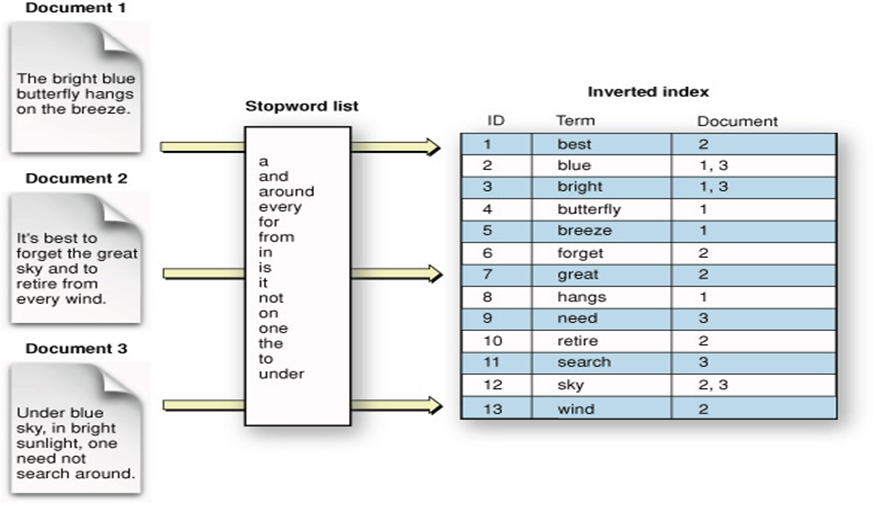
\includegraphics[width=1\textwidth]{figures/inverted_index.png}
\caption{Inverted index in Elasticsearch. \cite{elastic_sharding}}
\label{fig:inverted_index}
\end{figure}

We can look at the data from different levels of abstraction. In the Elasticsearch, there are more or less these levels of abstractions / concepts when we talk about data and structure:

\begin{enumerate}[noitemsep]
\item fields
\item documents
\item mapping
\item mapping types (legacy)
\item index
\item shards, replicas, nodes, cluster
\item analyzers \cite{elastic_concepts}
\end{enumerate}

\subsection{Fields}

Fields are the smallest units of data in Elasticsearch. A field is simply a key inside the JSON document, which has a corresponding value. The value can be of various \textit{field data types}. There are numerous data types in Elasticsearch. From simple \texttt{boolean} or \texttt{integer} to spatial data types like \texttt{geo\_point}. If we do not define a mapping for the fields, the data types are derived from the JSON document itself. We will talk about this more in Section \ref{sssec:mapping}.

A single field can have multiple data types. This is a concept of \textit{multi-fields} in Elasticsearch. For example, a \texttt{string} field could be mapped as a \texttt{text} field for full-text search, and as a \texttt{keyword} field for sorting and aggregations.

\subsection{Documents}

Documents are considered as the base unit of the Elasticsearch storage. A document is simply a JSON object which is stored within an Elasticsearch index. We can compare the document to a single row inside the relational database table. The document consists of user-defined fields. Some reserved fields are used as the document metadata. For example, the \texttt{\_id} field is automatically generated sequential identifier of a document. The metadata fields start with the underscore. A simple document could look like this:

\begin{code}
\begin{minted}{json}
{
  "_index" : "bank",
  "_type" : "_doc",
  "_id" : "1",
  "_version" : 1,
  "_seq_no" : 0,
  "_primary_term" : 1,
  "found" : true,
  "_source" : {
    "account_number" : 1,
    "balance" : 39225,
    "firstname" : "Amber",
    "lastname" : "Duke",
    "age" : 32,
    "gender" : "M",
    "address" : "880 Holmes Lane",
    "employer" : "Pyrami",
    "email" : "amberduke@pyrami.com",
    "city" : "Brogan",
    "state" : "IL"
  }
}
\end{minted}
\captionof{listing}{A simple Elasticsearch document.}
\label{code:sample_doc}
\end{code}

\subsection{Mapping}
\label{sssec:mapping}

Mapping is a process of defining the data types of the user-defined fields within an index. There are two types of mappings in Elasticsearch:

\begin{enumerate}[noitemsep]
\item dynamic mapping
\item explicit mapping
\end{enumerate}

\textbf{Dynamic mapping} is an automatic process of data types definition. The engine automatically detects and assigns the data types to the new fields. It uses default rules for this process, which can be configured by the users to precisely meet their expectations. For example, we could customize the way the engine detects date formats based on our preferences.

\textbf{Explicit mapping} is a process where the user explicitly defines the data types of the particular fields within an index. For example, we could define that an email should be of the \texttt{keyword} type since we do not need to use full-text search for the emails:

\begin{code}
\begin{minted}{json}
{
  "mappings": {
    "properties": { 
      "email":  { "type": "keyword"  }
  }
}
\end{minted}
\captionof{listing}{An example of the explicit mapping.}
\label{code:explicit_mapping}
\end{code}

\subsection{Mapping Types}

The mapping types were used to represent a type of indexed document. They were removed in version 7 of Elasticsearch. For this reason, we will not cover them in this article. If you want to learn more, please, refer to the \textit{Removal of mapping types} article \cite{mapping_types}.

\subsection{Index}

The index is considered the largest unit of data in Elasticsearch. It is a logical partition of documents and can be compared to a database or schema in the world of relational databases. The index can separate different types of documents and apply a specific configuration for the optimized collection of documents within an index. You can define as many indexes as you want. The indexes hold documents that are unique to each index.

\subsection{Shards, Replicas, Nodes \& Cluster}

There is no limit to how many documents you can store in one \textit{index}. A common issue with Elasticsearch is when your index becomes big enough, so it starts to exceed your machine's physical storage. This is a moment when we use a \textit{shard}.

There is an option to partition an index or multiple indexes into the shards. We call it horizontal partitioning. The concept is illustrated in Figure \ref{fig:sharding}.

\begin{figure}[h]
\centering
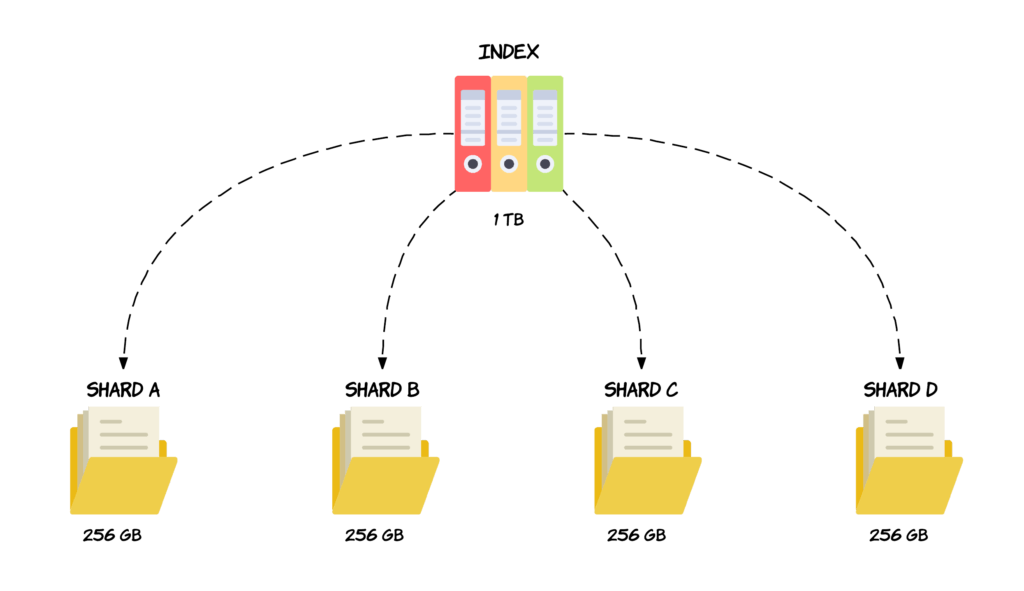
\includegraphics[width=1\textwidth]{figures/sharding.png}
\caption{Index split into multiple shards. \cite{understanding_sharding}}
\label{fig:sharding}
\end{figure}

Another logical partition is something called \textit{node}. Node is practically an instance of the Elasticsearch process. A collection of nodes is called \textit{cluster}. The partitioning is illustrated in Figure \ref{fig:cluster}.

\begin{figure}[t]
\centering
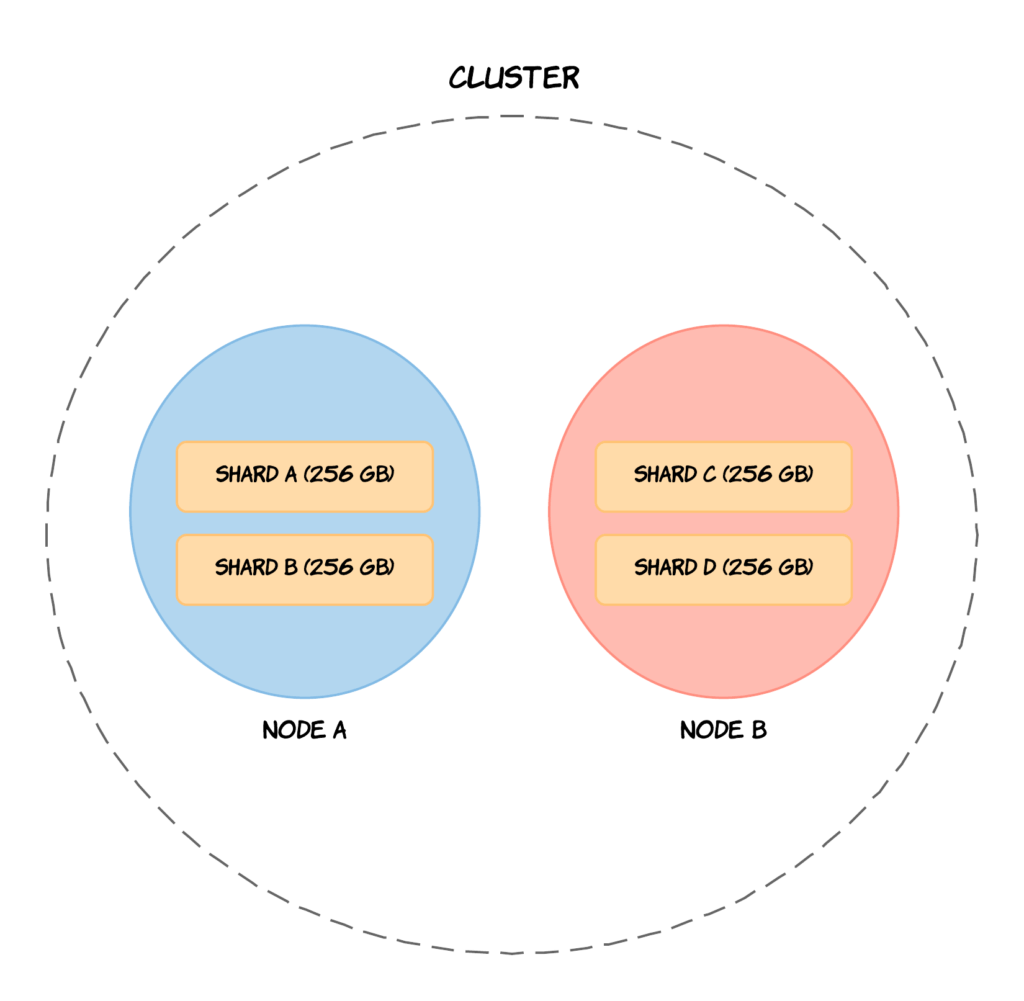
\includegraphics[width=.75\textwidth]{figures/cluster.png}
\caption{Cluster split into multiple nodes. \cite{understanding_sharding}}
\label{fig:cluster}
\end{figure}

One of the benefits of the nodes is the ability to distribute your system across multiple machines or physical storages. This is tightly connected with something called \textit{replica}. Replicas are copies of your index's shards. To ensure high availability, a replica is not stored on the same node as an original shard. This mechanism enables us to implement fail-safe mechanisms to prevent data loss in case of a failure.

All nodes know about all the other nodes in the cluster and can forward client requests to the appropriate node. There are multiple types of nodes in the engine which have different roles -- data node, machine learning node\dots

\subsection{Analyzers}

Analyzers are not directly connected to the structure of the Elasticsearch but are very important. They are utilities used during the indexing process to parse the full-text based on some grammar or tokenizer. By default, Elasticsearch applies \textit{Standard Analyzer} which is able to parse a common English text. The advantage is that you can define your analyzer or use some other already defined analyzers, e.g., if you tried to parse a text in the Klingon language.

\section{Query DSL}

Elasticsearch provides us with a simple (HTTP) REST API to manage our cluster, index, and search our data. It is a Domain Specific Language (DSL) we use to query the engine and work with it. To start using it, you can take advantage of any tool for sending HTTP requests, e.g., \textit{cURL} tool. Let's look at some simple examples of the API.

To add (index) some data, we simply run a \texttt{PUT} request with the payload we need:

\begin{code}
\begin{minted}{json}
PUT /languages/_doc/1
{
    "name": "Python"
}
\end{minted}
\captionof{listing}{An example of indexing some data.}
\label{code:indexing}
\end{code}

The request creates the index \texttt{languages} if it doesn't already exist. The \texttt{\_doc} is an important part of the path. In combination with the \texttt{PUT} method, we tell Elasticsearch that we want to create a new document. To query the document, we use the same path and \texttt{GET} method. We get the following response:

\begin{code}
\begin{minted}{json}
GET /languages/_doc/1
{
  "_index" : "languages",
  "_type" : "_doc",
  "_id" : "1",
  "_version" : 1,
  "_seq_no" : 10,
  "_primary_term" : 1,
  "found" : true,
  "_source" : {
    "name": "Python"
  }
}
\end{minted}
\captionof{listing}{The result of querying the data.}
\label{code:query_data}
\end{code}

If we want to search the \texttt{languages} index and sort the results, for example, by the name, we can use a simple query for it:

\begin{code}
\begin{minted}{json}
GET /languages/_search
{
  "query": { "match_all": {} },
  "sort": [
    { "name": "asc" }
  ]
}
\end{minted}
\captionof{listing}{Searching and sorting the data.}
\label{code:search_data}
\end{code}

This will return the languages sorted by their name. By default, the engine returns only the first 10 documents that match the search criteria. We can adjust this behavior by adding additional parameters to the query. You can note that we define the request body in the \texttt{GET} method. Many of you could argue that this goes against the REST principles, but it is the way the DSL is defined.

If you want to learn more about the DSL, please refer to the \textit{Query DSL} \cite{query_dsl} section of the official Elasticsearch documentation.

\section{Elastic Stack (ELK)}

\textit{Elastic Stack (ELK)} is a set of tools that are often used to enhance the work with Elasticsearch. In addition to the engine itself, you can find here the tools like Kibana, Logstash, and Beats.

\textbf{Kibana} is an open-source analytics and visualization platform designed to work with Elasticsearch. We can use it to search, index, view, and generally interact with our data stored in Elasticsearch indexes. It enables us to visualize data, generate reports with a variety of charts, tables, maps\dots

\textbf{Logstash} is a powerful data parsing and transformation tool. It is a recommended addition to Elasticsearch if you want to do complex and advanced transformations over your data.

\textbf{Beats} are open source data shippers that you install as autonomous agents/services on your OS. They send operational data to Elasticsearch. Each Beat can be installed separately. We can use them, for example, to collect the system metrics (CPU, RAM\dots) and send them to Elasticsearch. We can also use them in combination with Logstash to parse or transform the data before sending them to the engine.

To learn more about ELK, please refer to the \textit{Getting started with the Elastic Stack} \cite{elastic_stack} section of the official Elasticsearch documentation.

\newpage

\section*{Conclusion}
\addcontentsline{toc}{section}{Conclusion}

\textit{Elasticsearch} and \textit{ELK} are powerful tools that enable us to use near real-time full-text search over the documents. The main characteristic is the schema-free way of how the engine stores the data. It gives us the freedom to manipulate large sets of heterogeneous data. It also obligates us to handle the data manipulation on the application level properly.

In the first section, we described the main structure and principles of the Elasticsearch engine. We showed different levels of abstractions from the particular fields of the document, through the index, up to the cluster itself composed of different nodes, shards, indexes\dots

In the second section, we made a brief preview of the basic syntax of the query DSL. We described that the engine can be queried through the specific REST API and showed how we can take advantage of the HTTP protocol, methods, and DSL to work with the engine.

In the last section, we looked at the Elastic Stack (ELK). ELK is a set of tools that are designed to work smoothly with Elasticsearch. We described \textit{Kibana} (analytics and visualization platform), \textit{Logstash} (parsing and transformation tool), and \textit{Beats} (set of data shippers).

This article aimed to show the basic concepts, characteristics, and tools connected with Elasticsearch. It should serve you as a kick-off and inspiration for your next project where you would think about implementing a fast, near real-time search.

\newpage
\printbibliography
\addcontentsline{toc}{section}{References}

\end{document}
